\documentclass[12pt,a4paper]{report}
\usepackage[utf8]{inputenc}
\usepackage[T1]{fontenc}
\usepackage[english]{babel}
\usepackage{graphicx}
\usepackage{geometry}
\usepackage{fancyhdr}
\usepackage{listings}
\usepackage{xcolor}
\usepackage[hidelinks]{hyperref}
\usepackage{float}
\usepackage{tikz}
\usepackage{titlesec}

% Reduce spacing for titles
\titleformat{\chapter}[display]
  {\normalfont\huge\bfseries}{\chaptertitlename\ \thechapter}{10pt}{\Huge}
\titlespacing*{\chapter}{0pt}{-30pt}{15pt}
\titlespacing*{\section}{0pt}{10pt}{5pt}
\titlespacing*{\subsection}{0pt}{10pt}{5pt}
\titlespacing*{\subsubsection}{0pt}{10pt}{5pt}

\usepackage{setspace}
\usepackage{caption}
\usepackage{subcaption}
\usepackage{lipsum}
\usepackage{array}

% Colors
\definecolor{codegreen}{rgb}{0,0.6,0}
\definecolor{codegray}{rgb}{0.5,0.5,0.5}
\definecolor{codepurple}{rgb}{0.58,0,0.82}
\definecolor{backcolour}{rgb}{0.95,0.95,0.92}
\definecolor{EMSIGreen}{RGB}{0,102,51}
\definecolor{EMSILightGreen}{RGB}{144,238,144}

\geometry{
    a4paper,
    top=25mm,
    bottom=25mm,
    left=25mm,
    right=25mm
}

\setlength{\parskip}{1em}
\onehalfspacing

% Listing Configuration
\lstdefinestyle{cppstyle}{
    backgroundcolor=\color{backcolour},   
    commentstyle=\color{codegreen},
    keywordstyle=\color{blue},
    numberstyle=\tiny\color{codegray},
    stringstyle=\color{codepurple},
    basicstyle=\ttfamily\footnotesize,
    breakatwhitespace=false,         
    breaklines=true,                 
    captionpos=b,                    
    keepspaces=true,                 
    numbers=left,                    
    numbersep=5pt,                  
    showspaces=false,                
    showstringspaces=false,
    showtabs=false,                  
    tabsize=4,
    language=C++,
    frame=single,
    rulecolor=\color{black}
}

\lstset{style=cppstyle}

% Headers and Footers
\pagestyle{fancy}
\fancyhf{}
\lhead{MediaForge System}
\rhead{\leftmark}
\cfoot{\thepage}

\begin{document}

% ================= COVER PAGE =================
\begin{titlepage}
\thispagestyle{empty}

\definecolor{EMSIGreen}{RGB}{0, 102, 51}

% ---------- BACKGROUND EMSI EXACT ----------

\begin{tikzpicture}[remember picture,overlay]

% ================= LEFT VERTICAL BAND =================
\fill[EMSIGreen]
(current page.north west) rectangle
([xshift=2cm]current page.south west);

% ================= BOTTOM-LEFT white BAR =================
\fill[white]
([xshift=0cm,yshift=1cm]current page.south west) rectangle
([xshift=8cm,yshift=3cm]current page.south west);

% ================= BOTTOM-LEFT GREEN BAR =================
\fill[EMSIGreen]
([xshift=0cm,yshift=2.3cm]current page.south west) rectangle
([xshift=10.5cm,yshift=1.2cm]current page.south west);

% ================= BOTTOM-RIGHT TRIANGLE DECORATION =================
\fill[EMSIGreen]
    (current page.south east) --
    ([xshift=-5cm]current page.south east) --
    ([ yshift=5cm]current page.south east)
    -- cycle;

% ================= LEVEL LABEL (BOTTOM-LEFT) =================
\node[anchor=west, text=white, font=\bfseries\small]
at ([xshift=0.7cm,yshift=1.8cm]current page.south west)
{3\textsuperscript{rd} Year Computer Engineering and Networks};

\end{tikzpicture}
% ---------- CONTENT ----------
\centering
\vspace*{0.5cm} 


\includegraphics[width=0.4\textwidth]{logo-1.png}\\[0.2cm] 

\textbf{Moroccan School of Engineering Sciences of Tangier}

\vspace{1.2cm}

{\Large\bfseries END OF MODULE PROJECT}\\[0.4cm]

{\large Department}\\[0.1cm]
{\bfseries Computer Engineering and Networks (3IIR)}\\[0.8cm]

{\large Project Title}\\[0.3cm]

\fbox{
  \parbox{0.85\textwidth}{
    \centering
    \Large\bfseries
    Design and Development of a Multimedia Library Management System (MediaForge)
  }
}

\vspace{1cm}

{\large Realized by: }\\[0.2cm]
\textbf{
Nizar EL IDRYSY
}

\vspace{0.8cm}

\begin{flushleft}
\textbf{Academic Supervisor}\\
Pr. Youssef JDIDOU
\end{flushleft}

\vspace{0.6cm}

\begin{center}
\textbf{Jury Members}\\
Pr. Youssef JDIDOU
\end{center}

\vfill
\begin{center}
{\large Submission Date: January 7, 2026}
\end{center}

\vfill
\end{titlepage}

% ================= DEDICATION =================
\chapter*{Dedication}
\addcontentsline{toc}{chapter}{Dedication}
\vspace*{3cm}
\begin{center}
    \itshape\Large
    \textbf{To our dearest professor, Mr. Youssef JDIDOU,}
    
    \vspace{1cm}
    For his invaluable kindness, enlightened guidance, and exceptional pedagogy that transformed our learning into a true passion. This project is a modest testimony of our gratitude for your constant dedication to our academic and professional success.
    
    \vspace{1cm}
    \textbf{To our parents,}
    
    \vspace{0.5cm}
    Sources of our motivation and unwavering support, who never ceased to believe in us. No words can express our gratitude for your sacrifices.
    
    \vspace{1cm}
    To all our friends and colleagues of the 3IIR class, with whom we share this engineering adventure.
\end{center}
\vfill

% ================= ACKNOWLEDGEMENTS =================
\chapter*{Acknowledgements}
\addcontentsline{toc}{chapter}{Acknowledgements}

Before beginning this report, we would like to extend our deepest thanks to all those who contributed, directly or indirectly, to the realization of this project.

First and foremost, we warmly thank the administration of the \textbf{Moroccan School of Engineering Sciences (EMSI)} for providing us with a stimulating learning environment conducive to creativity and excellence.

We express our profound gratitude to our supervisor, \textbf{Pr. Youssef JDIDOU}, who guided us with patience and rigor. His wise advice on software architecture and C++ best practices was decisive in the success of this project. His lectures and practical sessions formed the solid foundation upon which we built this application.

Finally, we thank all those who participated in the testing phases of the application, allowing us to identify and correct imperfections to deliver a quality finished product.

% ================= TABLE OF CONTENTS =================
\tableofcontents

% ================= LIST OF FIGURES =================
\listoffigures
\addcontentsline{toc}{chapter}{List of Figures}

% ================= CHAPTER 1 =================
\chapter{General Introduction}

\section{Project Context}
The automation of management processes has become an inescapable necessity for any modern organization. In the educational and cultural sector, multimedia libraries play a central role as vectors of knowledge and entertainment. However, manual management of a large number of resources (books, DVDs, audio files, audiobooks) and users (students, professors, staff) quickly becomes a tedious task prone to human error.

It is in this context that our project \textbf{MediaForge System} falls. It is a technological response to the challenges faced by school multimedia library managers.

\section{Problem Statement}
How to design a computer system capable of efficiently managing the cycle of borrowing, the diversity of multimedia supports, and different user access levels, while remaining simple to use for non-expert users?

The main challenges are:
\begin{itemize}
    \item Diversity of media: A book does not have the same properties as a video (duration vs number of pages).
    \item Conflict management: A media item cannot be borrowed by two people simultaneously.
    \item Data security: User information must be protected.
    \item User experience: A console application can be austere; the challenge is to make it attractive.
\end{itemize}

\section{Project Objectives}
The goal of this project is to develop a complete application in C++ language that allows to:
\begin{enumerate}
    \item \textbf{Centralize data}: Group all media and users in a single system.
    \item \textbf{Automate tasks}: Availability calculation, basket management, search filtering.
    \item \textbf{Secure access}: Implementation of a robust authentication system.
    \item \textbf{Offer a friendly interface}: Use of colors and structured menus to guide the user.
\end{enumerate}

\section{Report Structure}
This document is structured to logically present the project progress:
\begin{itemize}
    \item \textbf{Chapter 2} analyzes the needs and specifies the features.
    \item \textbf{Chapter 3} details the technical architecture and UML design.
    \item \textbf{Chapter 4} dives into code implementation and error handling.
    \item \textbf{Chapter 5} presents the final results through usage scenarios.
\end{itemize}

% ================= CHAPTER 2 =================
\chapter{Analysis and Requirements Specification}

\section{Actor Identification}
System analysis allowed identifying two main actors interacting with the application.

\subsection{The Administrator}
The administrator is the library manager. They possess the highest privileges. Their role is to keep the system operational and up to date.
Their responsibilities include:
\begin{itemize}
    \item Creation of new user accounts (students or other administrators).
    \item Deletion of obsolete accounts.
    \item Catalog supervision (adding/removing media - simulated by file reading).
    \item Consultation of global statistics (number of loans, media popularity).
\end{itemize}

\subsection{The Client (Member)}
The client represents the standard end user, usually a student or a teacher.
They use the system to:
\begin{itemize}
    \item Search for books or multimedia files.
    \item Build a borrowing basket.
    \item Validate loans or make purchases.
    \item Consult their personal history.
\end{itemize}

\section{Functional Requirements Specification}

\subsection{Global Use Case}
Although this report does not contain a formal graphical UML diagram, we can textually describe the major use cases:

\subsubsection{Case N°1: Authentication}
\textbf{Actor}: All.
\textbf{Description}: The user must enter a valid email and password.
\textbf{Alternative flow}: If credentials are incorrect, the system denies access and emits an audible alert.

\subsubsection{Case N°2: Basket Management}
\textbf{Actor}: Client.
\textbf{Description}: The user navigates the catalog, selects an item, and adds it to their temporary basket. They can then validate the basket to transform the content into real loans.

\subsubsection{Case N°3: Media Search}
\textbf{Actor}: All.
\textbf{Description}: The user enters a string. The system scans the database and displays all media whose title contains the entered string (case insensitive).

\section{Technical and Environmental Constraints}
To ensure portability and performance, the following constraints were respected:
\begin{itemize}
    \item \textbf{Language}: C++ (Standard 17) for its fine memory management and execution speed.
    \item \textbf{Interface}: Console (CLI) compatible with Unix (macOS/Linux) and Windows terminals.
    \item \textbf{Storage}: Text files (.txt) for maximum portability without dependence on a complex database server (like SQL Server or Oracle).
\end{itemize}

% ================= CHAPTER 3 =================
\chapter{Architecture and Design}

\section{Object-Oriented Paradigm}
The choice of Object-Oriented Programming (OOP) is strategic. It allows modeling the real world intuitively. A library is composed of objects (Books, Users) that interact with each other.

\subsection{Inheritance}
Inheritance allowed us to factorize code. Instead of rewriting \texttt{title} and \texttt{price} attributes for each media type, we defined them in a parent class \texttt{Media}.

\begin{figure}[H]
    \centering
    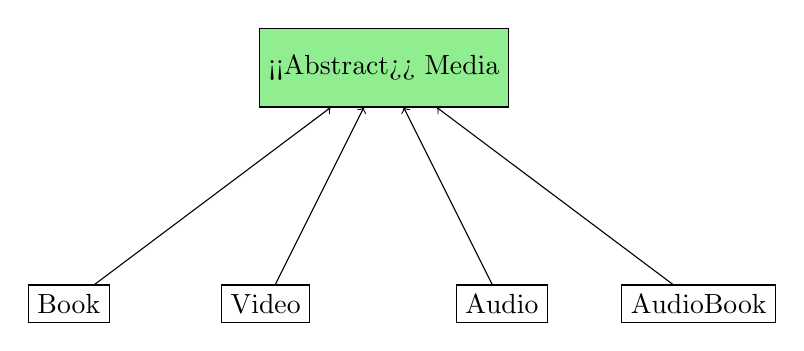
\begin{tikzpicture}[node distance=2cm]
    \node (Media) [draw, rectangle, minimum width=3cm, minimum height=1cm, fill=EMSILightGreen] {<<Abstract>> Media};
    \node (Book) [draw, rectangle, below of=Media, xshift=-4cm, yshift=-1cm] {Book};
    \node (Video) [draw, rectangle, below of=Media, xshift=-1.5cm, yshift=-1cm] {Video};
    \node (Audio) [draw, rectangle, below of=Media, xshift=1.5cm, yshift=-1cm] {Audio};
    \node (AudioBook) [draw, rectangle, below of=Media, xshift=4cm, yshift=-1cm] {AudioBook};
    
    \draw[->] (Book) -- (Media);
    \draw[->] (Video) -- (Media);
    \draw[->] (Audio) -- (Media);
    \draw[->] (AudioBook) -- (Media);
    \end{tikzpicture}
    \caption{Media Class Hierarchy}
\end{figure}

As illustrated above, \texttt{AudioBook} is a hybrid class (representing the flexibility of our polymorphic design).

\subsection{Polymorphism}
Polymorphism is used extensively. The \texttt{displayCompact()} method is virtual in the \texttt{Media} class and implemented differently in each subclass. This allows displaying a heterogeneous list of media (Books and Videos mixed) by calling the same method, with the system dynamically determining which version to execute.

\section{Data Structures}

\subsection{Memory Management with Smart Pointers}
In modern C++ (C++11 and later), manual memory management with \texttt{new} and \texttt{delete} is discouraged as it is a source of errors (memory leaks). We opted for \texttt{std::shared\_ptr}.

\begin{itemize}
    \item \textbf{Advantages}: Automatic memory release when the object is no longer used.
    \item \textbf{Application}: Library vectors contain \texttt{shared\_ptr<Media>}.
\end{itemize}

\subsection{File System}
The persistence architecture relies on three pillars:
\begin{enumerate}
    \item \textbf{users.txt}: Account database.
    \item \textbf{owned.txt}: Association table between users and borrowed media.
    \item \textbf{baskets.txt}: Temporary backup of baskets in progress.
\end{enumerate}

This approach allows restarting the application without losing the state of transactions.

% ================= CHAPTER 4 =================
\chapter{Implementation and Development}

This chapter presents the most relevant technical aspects of the source code. The full project contains over 1200 lines of code; we will focus on key mechanisms.

\section{The UI Class: A Textual Graphics Engine}
To offer a user experience superior to a simple black and white console, we developed a static \texttt{UI} class.

\subsection{ANSI Color Management}
ANSI escape codes allow controlling text and background color in the terminal.
\begin{lstlisting}[caption={ANSI Color Macros Definitions}]
#define ansiReset "\033[0m\033[40m"
#define bold "\033[1m"
#define highlightBlue "\033[44m"
#define highlightGreen "\033[42m"
\end{lstlisting}

\subsection{Loading Animation}
A \texttt{slowPrint} function was created to simulate text being typed character by character, giving a "hacker" or "system processing" effect.

\begin{lstlisting}[caption={Typewriter Effect Function}]
static void slowPrint(string text, int speedMs) {
    for (size_t i = 0; i < text.length(); ++i) {
        cout << text[i] << flush;
        this_thread::sleep_for(chrono::milliseconds(speedMs));
    }
}
\end{lstlisting}

\section{Core Business Logic}

\subsection{The User Class}
This class encapsulates all personal data and possible actions of a user. Note the use of \texttt{vector} to store \texttt{Media} objects.

\begin{lstlisting}[caption={User Class Extract}]
class User {
protected:
    string email;
    string password;
    string role;
    vector<shared_ptr<Media>> basket;
    vector<shared_ptr<Media>> ownedMedia;

public:
    void addToBasket(shared_ptr<Media> m) {
        if(m->getIsBorrowed()) {
             cout << "Item is currently borrowed." << endl;
             return;
        }
        basket.push_back(m);
        cout << "Added to basket." << endl;
    }
};
\end{lstlisting}

\subsection{Search Engine}
The search functionality is crucial for ergonomics. It is implemented with linear complexity $O(N)$.

\begin{lstlisting}[caption={Search Algorithm}]
void searchMedia(const vector<shared_ptr<Media>>& library) {
    string query;
    UI::inputLine(query);
    string lowerQuery = toLower(query);
    
    for(const auto& m : library) {
        // Case insensitive substring search
        if(toLower(m->getTitle()).find(lowerQuery) != string::npos) {
            results.push_back(m);
        }
    }
    // Display results...
}
\end{lstlisting}

\section{Error Handling and Robustness}
An aspect often overlooked in student projects, but central to ours, is Error Handling. An application must never crash due to unexpected user input.

\subsection{Securing Numeric Inputs}
The classic `cin >> int` problem is that if the user enters a letter, the input stream blocks and the program enters an infinite loop.
We solved this with the \texttt{inputInt} method:

\begin{lstlisting}[caption={Secure Integer Input}]
static void inputInt(int& var) {
    string line;
    getline(cin, line); // Read the whole line as text
    try {
        if(line.empty()) { var = -1; return; }
        var = stoi(line); // Explicit String to Int conversion
    } catch (...) {
        var = -1; // Return invalid code on error
    }
}
\end{lstlisting}
Thanks to this method, if the user types "abc" instead of "123", the program continues normally displaying an "Invalid choice" message.

\subsection{Missing File Handling}
At startup, the application checks for the existence of data files. If they are missing, they are automatically created (\texttt{scanDirectory} method and \texttt{System} constructor). This avoids "File Not Found Exception" type errors.

% ================= CHAPTER 5 =================
\chapter{Results Presentation}
This section presents the final rendering of the application as it appears to the user.

\section{Home Interface}
The home screen was designed to be visually striking. It uses a complex ASCII frame representing a server or central terminal.

\begin{figure}[H]
    \centering
    \fbox{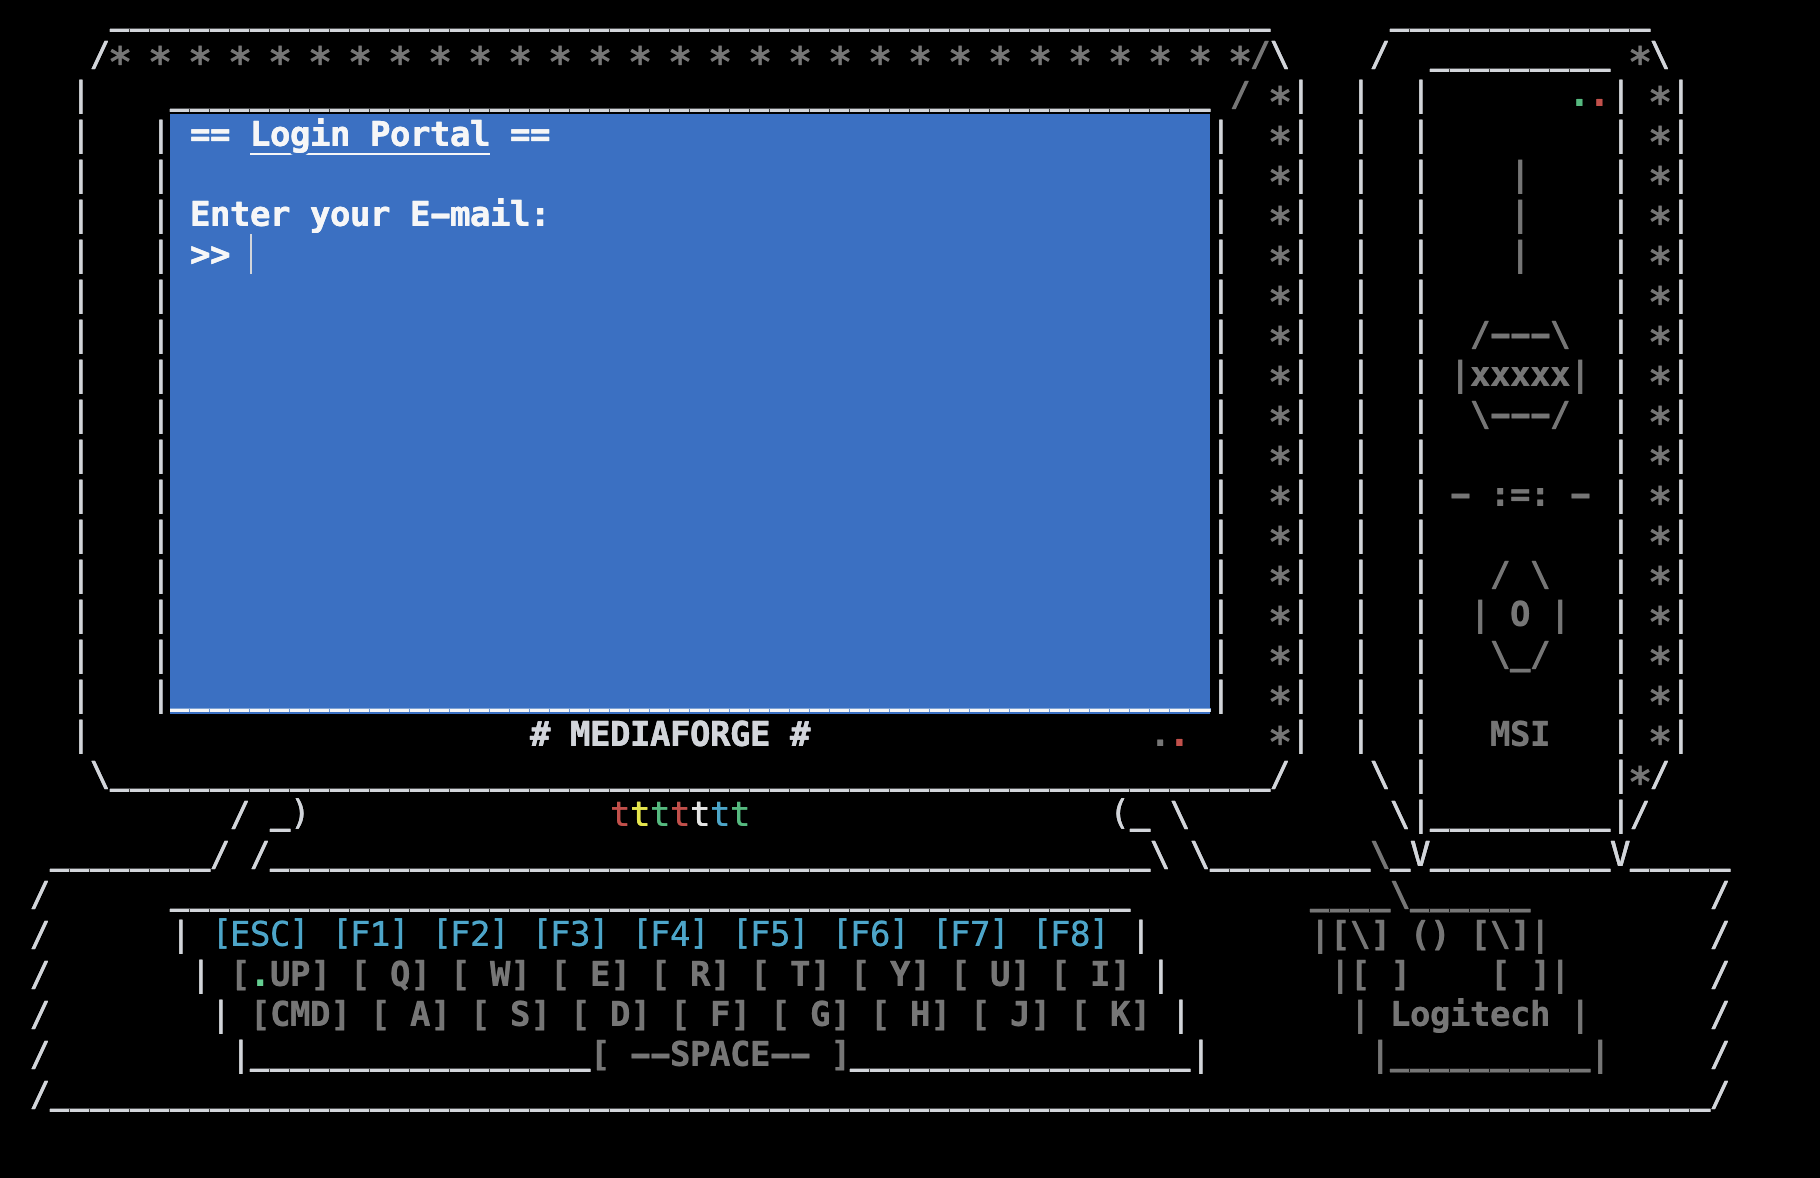
\includegraphics[width=0.9\textwidth]{home.png}}
    \caption{System Login Interface}
    \label{fig:home}
\end{figure}

As shown in Figure \ref{fig:home}, the user is immediately immersed in the application universe. Input fields appear sequentially.

\section{Client The dashboard}
Once authenticated successfully (the system plays a "success.mp3" sound), the client accesses their dashboard.

\begin{figure}[H]
    \centering
    \fbox{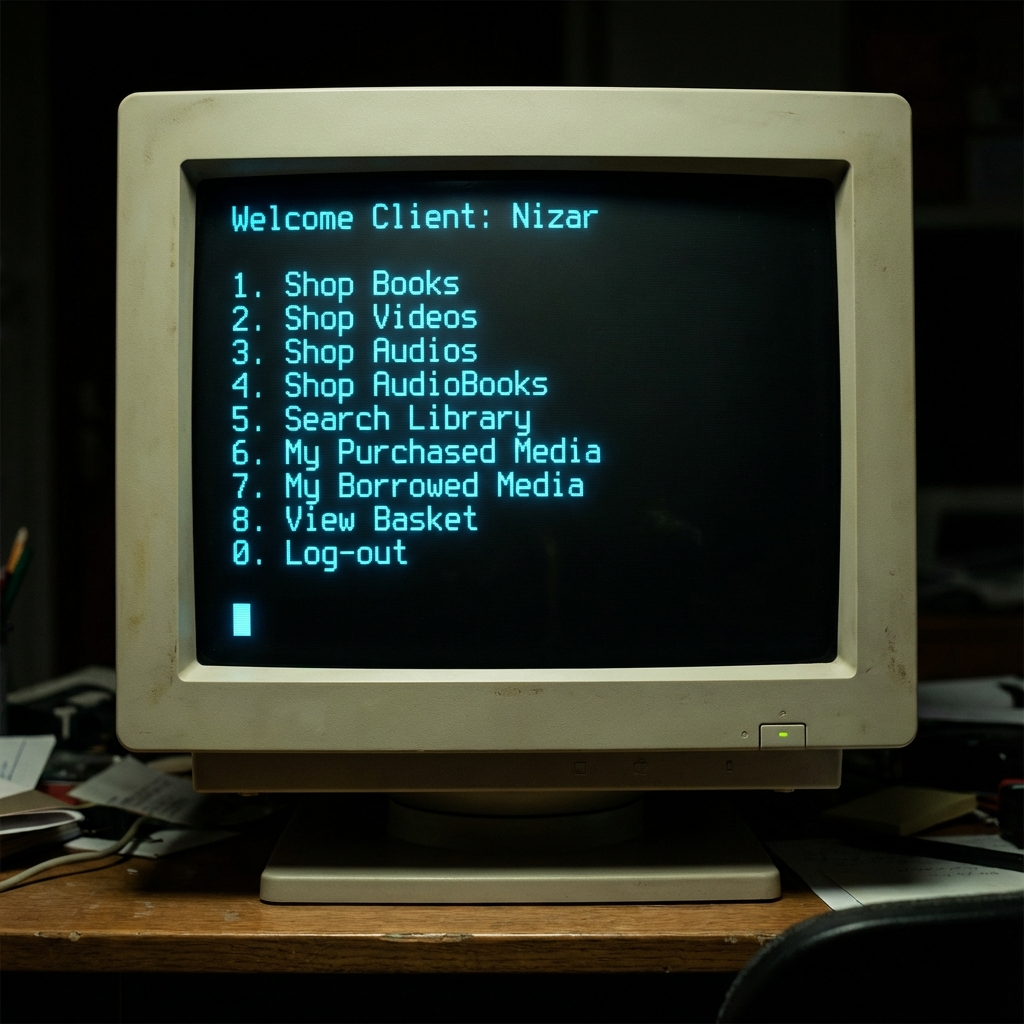
\includegraphics[width=0.9\textwidth]{menu.png}}
    \caption{Client Main Menu with Navigation Options}
    \label{fig:menu}
\end{figure}

The menu (Figure \ref{fig:menu}) clearly displays all available actions. The use of neon blue on specific backgrounds reduces eye strain and recalls professional development interfaces.

\section{Test Scenario: Purchasing Media}
Here is the typical flow of a purchase session:
\begin{enumerate}
    \item The client selects "1. Shop Books".
    \item The list of available books is displayed. Borrowed books are marked in \textcolor{red}{Red}, available ones in \textcolor{green}{Green}.
    \item The client enters the book number. It is added to the basket.
    \item The client goes to "8. View Basket". They see their order total.
    \item They select "Confirm Loan" or "Buy". If "Buy" is chosen, the media is marked as purchased and added to their "My Purchased Media" list.
\end{enumerate}

\section{Test Scenario: Administration}
The administrator has a different menu. They can:
\begin{itemize}
    \item View the list of all registered users.
    \item Delete a problematic user.
    \item Export a global report in \texttt{report.txt} format containing the stock status at a given time.
\end{itemize}

% ================= CONCLUSION =================
\chapter{General Conclusion and Outlook}

\section{Project Assessment}
At the end of this project, we successfully designed and developed a complete multimedia library management application, named \textbf{MediaForge System}.

Technically, this project allowed us to consolidate our skills in:
\begin{itemize}
    \item \textbf{C++ Language}: Mastery of syntax, pointers, references, and STL.
    \item \textbf{Object Design}: Concrete application of abstraction, encapsulation, and polymorphism concepts.
    \item \textbf{Algorithmics}: Implementation of efficient sorting and searching algorithms.
    \item \textbf{Project Management}: Teamwork and source code management.
\end{itemize}

The initial objective, which was to provide a tool automating loan management while remaining accessible, is fully achieved. The user interface, although in console mode, offers surprising ergonomics thanks to the care given to design.

\section{Current Limitations}
Despite its qualities, the system has certain limitations inherent to its nature as an academic project:
\begin{itemize}
    \item The absence of a Graphical User Interface (GUI) may deter some non-tech-savvy users.
    \item Text file storage is not suitable for very large scale (millions of users) due to performance and security reasons.
    \item The application is single-user (no real client-server mode via network).
\end{itemize}

\section{Future Improvements}
To evolve this project towards a professional solution, several avenues are conceivable:
\begin{enumerate}
    \item \textbf{Migration to an SQL Database}: Use SQLite or MySQL to secure and accelerate data access.
    \item \textbf{GUI Development}: Use the Qt framework to create an interface with mouse, buttons, and real book cover images.
    \item \textbf{Web Version}: Transform the C++ core into a backend (with a framework like Drogon) and create a Web frontend for remote accessibility.
    \item \textbf{Networking}: Implement a client-server architecture using sockets to allow multiple users to connect simultaneously from different machines.
\end{enumerate}

In conclusion, \textbf{MediaForge System} constitutes a solid and scalable foundation, demonstrating the power of C++ to create performant management applications.

% ================= BIBLIOGRAPHY =================
\chapter*{Bibliography and Webography}
\addcontentsline{toc}{chapter}{Bibliography and Webography}

\section*{Books}
\begin{enumerate}
    \item Bjarne Stroustrup, \textit{The C++ Programming Language}, 4th Edition, Addison-Wesley, 2013.
    \item Scott Meyers, \textit{Effective Modern C++}, O'Reilly Media, 2014.
\end{enumerate}

\section*{Websites Consulted}
\begin{itemize}
    \item \textbf{cppreference.com}: Official C++ standard library documentation.
    \item \textbf{stackoverflow.com}: For specific problem solving related to clang compilation errors.
    \item \textbf{overleaf.com}: For LaTeX report writing and compilation.
\end{itemize}

\end{document}
